\documentclass[12pt, twoside]{article}
\usepackage[letterpaper, margin=1in, headsep=0.5in]{geometry}
\usepackage[english]{babel}
\usepackage[utf8]{inputenc}
\usepackage{amsmath}
\usepackage{amsfonts}
\usepackage{amssymb}
\usepackage{tikz}

\usepackage{pgfplots}
\pgfplotsset{width=9cm,compat=1.9}

\usepackage{venndiagram}

\usepackage{graphicx}
\usepackage{enumitem}
\usepackage{multicol}

\usepackage{fancyhdr}
\pagestyle{fancy}
\fancyhf{}
\renewcommand{\headrulewidth}{0pt} % disable the underline of the header

\fancyhead[LE]{\thepage}
\fancyhead[RO]{\thepage \\ Name: \hspace{4cm} \,\\}
\fancyhead[LO]{BECA / Dr. Huson / IB Mathematics\\* Unit 5: Polynomial functions\\* 13 February 2020}

\begin{document}
\begin{enumerate}
\subsubsection*{5.11 Exam: Quadratic functions and their graphs (no calculator)}
  \item A quadratic function $f$ is shown with $x$-intercepts of $1$ and $5$, and vertex $(3,-4)$.
    \begin{center}
    \begin{tikzpicture}[yscale=0.75]
        \foreach \x in {-1,1,2,3,4,5,6}
          \draw[shift={(\x,0)},color=black] (0pt,-3pt) -- (0pt,3pt) node[below]  {$\x$};
        %\foreach \y in {-5,-4,-3,-2,-1,1,2,3}
          %\draw[shift={(0,\y)},color=black] (2pt,0pt) -- (-2pt,0pt) node[left]  {$\y$};
          \draw [thick, ->] (-2.5,0) -- (+6.5,0) node [right] {$x$};
          \draw [thick, ->] (0,-4.5) -- (0,6.5) node [right] {$y$};
        %\fill (1,-4.5) circle[radius=2pt] node [below] {$P$};
        %\fill (0,-4) circle[radius=2pt] node [right] {$Q$};
        \draw [<->] plot[domain= -0.25:5.5] (\x, {1*(\x-1)*(\x-5)});
    \end{tikzpicture}
    \end{center}
    The function $f$ can be written in the form $f(x)=(x-h)^2 +k$.
    \begin{enumerate}%[itemsep=0.8cm]
      \item Write down $h$ and $k$. \hfill [2] \\[0.5cm]
      The function can also be written in the form $f(x)=(x-a)(x-b)$
      \item Write down the value of $a$ and $b$. \hfill [2]
      \item Find the $y$-intercept. \hfill [2]
    \end{enumerate}
    \begin{tikzpicture}
      \draw (0,0) rectangle (15.2,8);
      \draw (8,0) rectangle (15.2,4.5);
      \node at (0,8)[below right]{\textbf{Working:}};
      \node at (8,4.5)[below right]{\textbf{Answers:}};
      \draw [dotted] (9,2.9)node[left]{(a)}--(15,2.9);
      \draw [dotted] (9,1.7)node[left]{(b)}--(15,1.7);
      \draw [dotted] (9,0.5)node[left]{(c)}--(15,0.5);
  \end{tikzpicture}

\newpage

  \item The diagram below shows part of the graph of the function $f(x)=x^2$.
    \begin{center}
    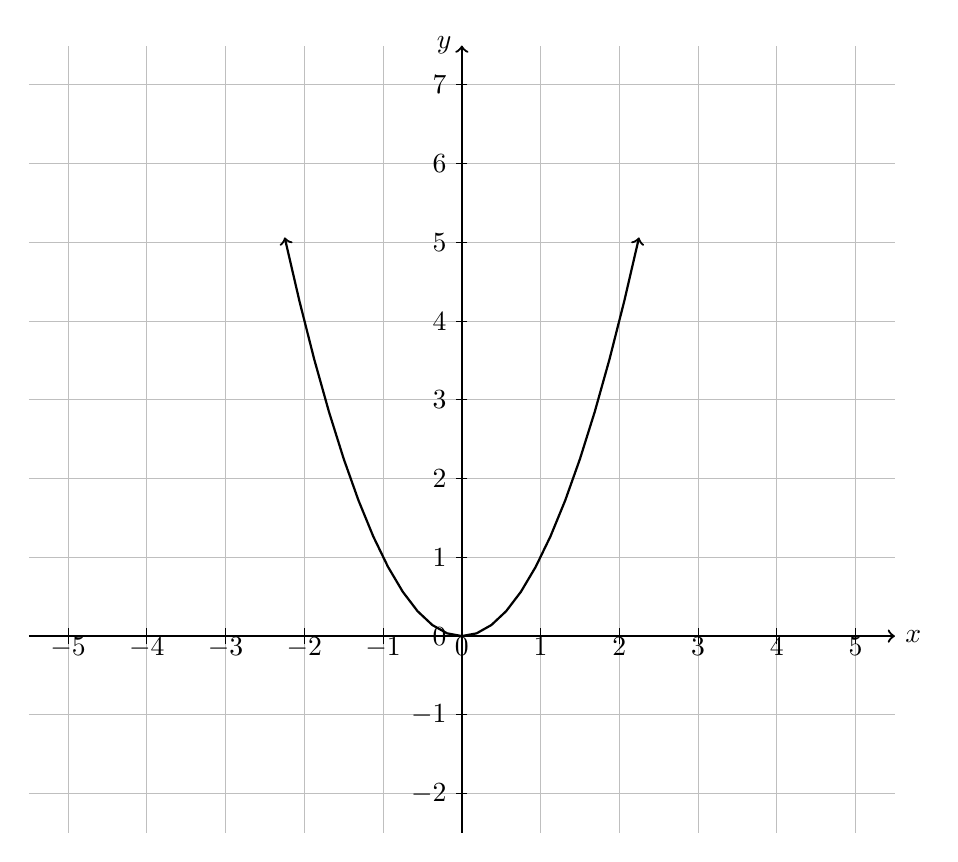
\begin{tikzpicture}
      \draw [thin, color=lightgray,, xstep=1.0cm,ystep=1.0cm] (-5.5,-2.5) grid (5.5,7.5);
      %\draw [thin, color=lightgray,, xstep=0.2cm,ystep=0.2cm] (-5.5,-1.5) grid (5.5,16.5);
      \foreach \x in {-5, -4, -3, -2, -1, 0,1,2,3,4,5}
      \draw[shift={(\x,0)},color=black] (0pt,-3pt) -- (0pt,3pt) node[below]  {$\x$};
      \foreach \y in {-2, -1, 0,1,2,3,4,5, 6,7}
      \draw[shift={(0,\y)},color=black] (2pt,0pt) -- (-2pt,0pt) node[left]  {$\y$};
      \draw [thick, ->] (-5.5,0) -- (+5.5,0) node [right] {$x$};
      \draw [thick, ->] (0,-2.5) -- (0,7.5) node [left] {$y$};
      \draw [thick, <->] plot[domain= -2.25:2.25] (\x, {(\x)*(\x)});
    \end{tikzpicture}
    \end{center}
    \begin{enumerate}
      \item $g(x)$ is the image of $f$ after a translation left 3 and up 1. Draw $g$.  \hfill [2]
      \item $g$ can be written in the form $g(x)=(x-h)^2 +k$. Write down $h$ and $k$.  \hfill [2]
      \item Expand $g$ to standard form, $g(x)=ax^2+bx+c$. \hfill [2]
    \end{enumerate}
      \begin{tikzpicture}
        \draw (0,0) rectangle (15.2,9);
        \draw (8,0) rectangle (15.2,3.5);
        \node at (0,9)[below right]{\textbf{Working:}};
        \node at (8,3.5)[below right]{\textbf{Answers:}};
        %\draw [dotted] (9,2.9)node[left]{(a)}--(15,2.9);
        \draw [dotted] (9,1.7)node[left]{(b)}--(15,1.7);
        \draw [dotted] (9,0.5)node[left]{(c)}--(15,0.5);
    \end{tikzpicture}

\newpage 
  \item %{[Maximum mark: 7]} \\[0.3cm]
  Let $f(x)=x^2+2x+1$ and $g(x)=x+1$.
      \begin{enumerate}
          \item Write down $f(0)$. \hfill [1]
          \item Find $(f - g)(x)$. \hfill [1]
          \item Find $(f \div g)(x)$ in simplest form, $x \neq 0$. \hfill [2]
          \item Write down $g^{-1}(4)$. \hfill [2]
          \item Find $g^{-1}(x)$. \hfill [2]
          \item Find $(f \circ g)(x)$. \hfill [2]
      \end{enumerate}
      \begin{tikzpicture}

          \draw (0,-1) rectangle (15.2,15);
          \draw (8,-1) rectangle (15.2,6.5);
          \node at (0,15)[below right]{\textbf{Working:}};
          \node at (8,6.5)[below right]{\textbf{Answers:}};
          \draw [dotted] (9,5)node[left]{(a)}--(15,5);
          \draw [dotted] (9,4)node[left]{(b)}--(15,4);
          \draw [dotted] (9,3)node[left]{(c)}--(15,3);
          \draw [dotted] (9,2)node[left]{(d)}--(15,2);
          \draw [dotted] (9,1)node[left]{(e)}--(15,1);
          \draw [dotted] (9,0)node[left]{(f)}--(15,0);
      \end{tikzpicture}

\newpage
  \item Let $f(x)=x^2-6x+7$. $f$ can be written in the form $f(x)=(x-h)^2 +k$.
    \begin{enumerate}
      \item Find the value of $h$ and of $k$. \hfill [2]
      \item Write down the equation of the axis of symmetry. \hfill [1]
      \item Find the solutions of $f(x)=0$. \hfill [2]
      \item Draw the function $f(x)$ on the grid below. \hfill [2]
  \end{enumerate}
    \begin{center}
      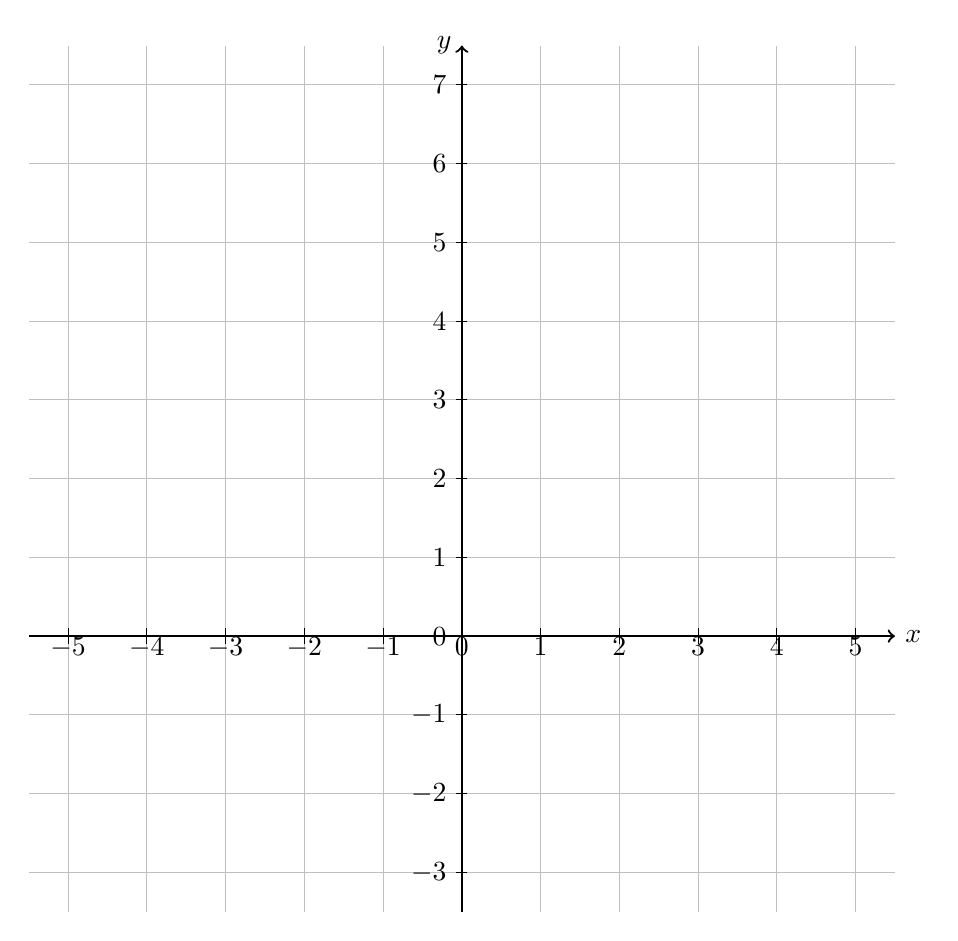
\begin{tikzpicture}
        \draw [thin, color=lightgray,, xstep=1.0cm,ystep=1.0cm] (-5.5,-3.5) grid (5.5,7.5);
        \foreach \x in {-5, -4, -3, -2, -1, 0,1,2,3,4,5}
        \draw[shift={(\x,0)},color=black] (0pt,-3pt) -- (0pt,3pt) node[below]  {$\x$};
        \foreach \y in {-3, -2, -1, 0,1,2,3,4,5, 6, 7}
        \draw[shift={(0,\y)},color=black] (2pt,0pt) -- (-2pt,0pt) node[left]  {$\y$};
        \draw [thick, ->] (-5.5,0) -- (+5.5,0) node [right] {$x$};
        \draw [thick, ->] (0,-3.5) -- (0,7.5) node [left] {$y$};
        \draw (3, 2);
        %\draw (1,1) circle[radius=2pt];
        %\fill (1,1) circle[radius=2pt];
        %\draw [<->] plot[domain= -0.25:6] (\x, \x*\x -6*\x + 7);  %.5*\x*\x -2*\x +3
      \end{tikzpicture}
    \end{center}
      \begin{tikzpicture}
        \draw (0,0) rectangle (15.2,7);
        \draw (8,0) rectangle (15.2,4.5);
        \node at (0,7)[below right]{\textbf{Working:}};
        \node at (8,4.5)[below right]{\textbf{Answers:}};
        \draw [dotted] (9,2.9)node[left]{(a)}--(15,2.9);
        \draw [dotted] (9,1.7)node[left]{(b)}--(15,1.7);
        \draw [dotted] (9,0.5)node[left]{(c)}--(15,0.5);
    \end{tikzpicture}
    
\newpage
  \item Consider $f(x)=x^2+qx+r$. The graph of $f$ has a minimum value when $x=-1.5$. The distance between the two zeros of $f$ is 9.
    \begin{enumerate}
      \item Show that the two zeros are 3 and $-6$. \hfill [2]
      \item Find the value of $q$ and $r$. \hfill [4]
    \end{enumerate}
      \begin{tikzpicture}
        \draw (0,0) rectangle (15.2,8);
        \draw (8,0) rectangle (15.2,2.5);
        \node at (0,8)[below right]{\textbf{Working:}};
        \node at (8,2.5)[below right]{\textbf{Answers:}};
        %\draw [dotted] (9,2.9)node[left]{(a)}--(15,2.9);
        %\draw [dotted] (9,1.7)node[left]{(b)}--(15,1.7);
        \draw [dotted] (9,0.5)node[left]{(b)}--(15,0.5);
    \end{tikzpicture}

  \item Consider the equation $x^2 + (k-2)x=-4$, where $k$ is a real number. Find the values of $k$ for which the equation has two equal real solutions.  \hfill [7]
  \begin{center}
    \begin{tikzpicture}
      \draw (0,0) rectangle (15.2,10);
      \draw (8,0) rectangle (15.2,2.5);
      \node at (0,10)[below right]{\textbf{Working:}};
      \node at (8,2.5)[below right]{\textbf{Answers:}};
      %\draw [dotted] (9,2.9)node[left]{(a)}--(15,2.9);
      %\draw [dotted] (9,1.7)node[left]{(b)}--(15,1.7);
      \draw [dotted] (9,0.5)node[left]{}--(15,0.5);
    \end{tikzpicture}
  \end{center}

\newpage
\item Let $f(x)=a(x+3)(x-1)$. The following diagram shows part of the graph of $f$.
\begin{center}
\begin{tikzpicture}[yscale=0.25]
    \foreach \x in {-3,1}
      \draw[shift={(\x,0)},color=black] (0pt,-15pt) -- (0pt,15pt);% node[below]  {$p$};
      \node at (-3,0)[below right]{$p$};
      \node at (1,0)[below left]{$q$};
    %\foreach \y in {-5,-4,-3,-2,-1,1,2,3}
      %\draw[shift={(0,\y)},color=black] (2pt,0pt) -- (-2pt,0pt) node[left]  {$\y$};
      \draw (-0.2,12)--(0.2,12)node[right]{12};
      \draw [thick, ->] (-3.5,0) -- (+2.5,0) node [right] {$x$};
      \draw [thick, ->] (0,-1.5) -- (0,15.5) node [right] {$y$};
    %\fill (1,-4.5) circle[radius=2pt] node [below] {$P$};
    %\fill (0,-4) circle[radius=2pt] node [right] {$Q$};
    \draw [<->] plot[domain= -3.1:1.1] (\x, {-4*(\x+3)*(\x-1)});
\end{tikzpicture}
\end{center}
The graph has $x$-intercepts at $(p,0)$ and $(q,0)$, and a $y$-intercept at $(0,12)$.
\begin{enumerate}%[itemsep=0.8cm]
  \item Write down the value of $p$ and of $q$. \hfill [2]
  \item Find the value of $a$. \hfill [3]
  \item Find the equation of the axis of symmetry of the graph of $f$. \hfill [3]
  \item Find the largest value of $f$.  \hfill [3]\\[0.25cm]
  The function $f$ can be written in the form $f(x)=a(x-h)^2 +k$.
  \item Write down the value of $h$ and $k$. \hfill [3]
\end{enumerate}
\begin{tikzpicture}
  \draw (0,-2.5) rectangle (15.2,9);
  \draw (9.2,-2.5) rectangle (15.2,4.5);
  \node at (0,9)[below right]{\textbf{Working:}};
  \node at (9.2,4.5)[below right]{\textbf{Answers:}};
  \draw [dotted] (10,2.9)node[left]{(a)}--(15,2.9);
  \draw [dotted] (10,1.7)node[left]{(b)}--(15,1.7);
  \draw [dotted] (10,0.5)node[left]{(c)}--(15,0.5);
  \draw [dotted] (10,-0.7)node[left]{(d)}--(15,-0.7);
  \draw [dotted] (10,-1.9)node[left]{(e)}--(15,-1.9);
\end{tikzpicture}


\end{enumerate}
\end{document}


\newpage
\item Graph the function $f(x)=x^2+2x+2$ over the domain $-1 \leq x\leq 1$.
\begin{itemize}
    \item[(a)] Mark points on the function representing $f(-1)=1$ and $f(1)=5$. Label them as coordinate pairs.
  \item[(b)] Graph and label the inverse of $f$, $f^{-1}(x)$, on the same axes over the domain corresponding to the range of $f$ graphed. Mark the inverses of the points named in part (a), labeling them as coordinate pairs.
  \item[(c)] Write down the domain and range of $f^{-1}(x)$ in the space below. \vspace{2cm}
\end{itemize}
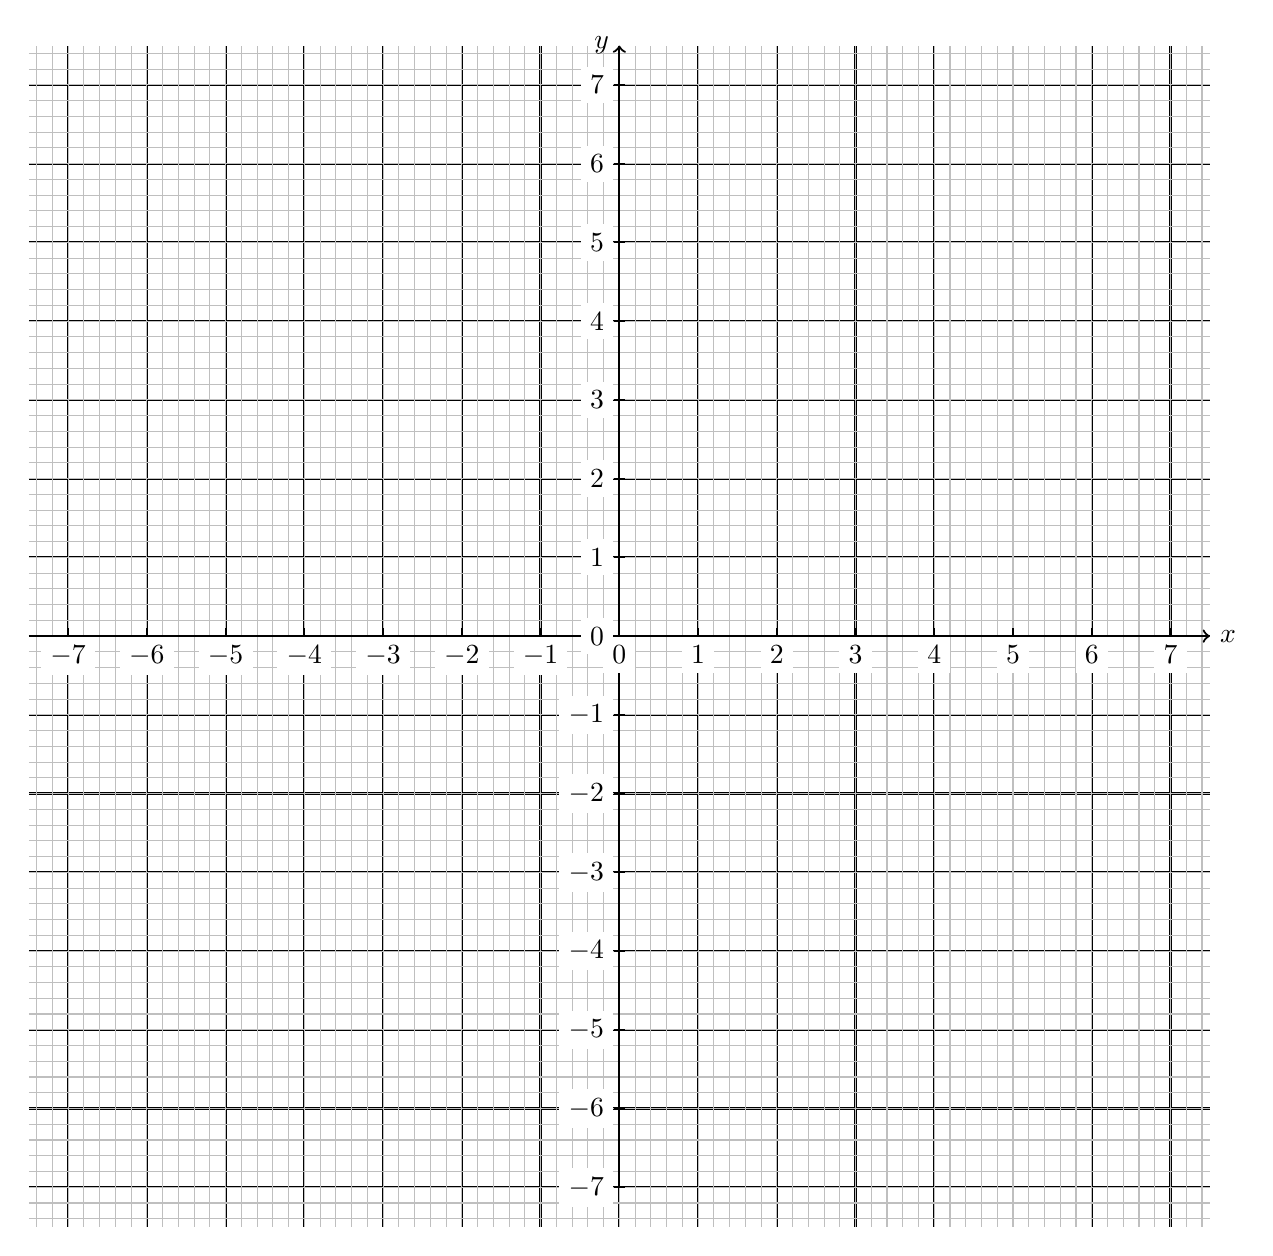
\begin{tikzpicture}[scale=1] %grid with numbered axes, IB cm paper.
  %\clip (-5.5, -1.5) rectangle (5.5, 7.5);
  \draw [thick, color=black,, xstep=1.0cm,ystep=1.0cm] (-7.5,-7.5) grid (7.5,7.5);
  \draw [thin, color=lightgray,, xstep=0.2cm,ystep=0.2cm] (-7.5,-7.5) grid (7.5,7.5);
  \draw [thick, ->] (-7.5,0) -- (+7.5,0) node [right] {$x$};
  \draw [thick, ->] (0,-7.0) -- (0,7.5) node [left] {$y$};
  \foreach \x in {-7,...,7}
    \draw[shift={(\x,0)},color=black] (0pt,-3pt) -- (0pt,3pt) node[below=3pt, fill=white]  {$\x$};
  \foreach \y in {-7,..., 7}
    \draw[shift={(0,\y)},color=black] (2pt,0pt) -- (-2pt,0pt) node[left, fill=white]  {$\y$};

  %\draw [<->, thick] plot[domain= -5:5] (\x, {(3*\x+1)/(\x-2)});
\end{tikzpicture}


\newpage


    \item The following diagram shows the graph of a function $f$.\\
      
\begin{tikzpicture}[scale=1] %grid with numbered axes, IB cm paper.
        %\clip (-5.5, -1.5) rectangle (5.5, 7.5);
        \draw [thick, color=black,, xstep=1.0cm,ystep=1.0cm] (-7.5,-7.5) grid (7.5,7.5);
        %\draw [thin, color=lightgray,, xstep=0.2cm,ystep=0.2cm] (-7.5,-7.5) grid (7.5,7.5);
        \draw [thick, ->] (-7.5,0) -- (+7.5,0) node [right] {$x$};
        \draw [thick, ->] (0,-7.0) -- (0,7.5) node [left] {$y$};
        \foreach \x in {-7,...,7}
          \draw[shift={(\x,0)},color=black] (0pt,-3pt) -- (0pt,3pt) node[below=3pt, fill=white]  {$\x$};
        \foreach \y in {-7,..., 7}
          \draw[shift={(0,\y)},color=black] (2pt,0pt) -- (-2pt,0pt) node[left, fill=white]  {$\y$};

        %\draw [<->, thick] plot[domain= -5:5] (\x, {(3*\x+1)/(\x-2)});
      \end{tikzpicture}
      \begin{enumerate}
        \item Find $f^{-1}(x)$.
        \item Find $(f \circ f)(-1)$.
        \item On the same diagram, sketch the graph of $y=-f(x)$.
      \end{enumerate}

    \item The following diagram shows part of the graph of a quadratic function $f$.

\newpage
    \item Consider the function $f(x)=x^2-6x-1$.
    \begin{enumerate}
        \item Sketch the graph of $f$, for $-4 \leq x \leq 3$.
        \item This function can also be written in the form $f(x)=(x-p)^2 -10$.\\*
        Write down the value of $p$.
        \item The graph of $g$ is obtained by reflecting the graph of $f$ in the $x$-axis, followed by a translation of $(0, 4)$.\\* Show that $g(x)=x^2+3x-1$.
        \item The graphs of $f$ and $g$ intersect at two points.\\*
        Write down the x-coordinates of these two points.
    \end{enumerate}




\begin{center}
  \begin{tikzpicture}
      \foreach \x in {-2, -1,1,2,3,4,5,6}
        \draw[shift={(\x,0)},color=black] (0pt,-3pt) -- (0pt,3pt) node[below]  {$\x$};
      \foreach \y in {-5,-4,-3,-2,-1,1,2,3}
        \draw[shift={(0,\y)},color=black] (2pt,0pt) -- (-2pt,0pt) node[left]  {$\y$};
        \draw [thick, ->] (-2.5,0) -- (+6.5,0) node [right] {$x$};
        \draw [thick, ->] (0,-5.5) -- (0,3.5) node [left] {$y$};
      %\fill (1,-4.5) circle[radius=2pt] node [below] {$P$};
      %\fill (0,-4) circle[radius=2pt] node [right] {$Q$};
      \draw [<->] plot[domain= -0.5:5.5] (\x, {1*(\x-1)*(\x-5)});
  \end{tikzpicture}
  \end{center}